\documentclass[12pt]{article}
\usepackage[utf8]{inputenc}
\usepackage{graphicx}
\usepackage[a4paper,includefoot,heightrounded,margin=1.2 in]{geometry}
\usepackage{adjustbox}
\usepackage{float}
\usepackage{array}
\usepackage{amsmath}
\begin{document}
\begin{titlepage}
\newcommand{\HRule}{\rule{\linewidth}{0.5mm}}

\center 

\textsc{\LARGE Lund University}\\[1.5cm] 
\textsc{\Large Physics Department }\\[0.5cm]
\textsc{\Large Atomic and Molecular Physics FYSC11}\\[0.5cm]


\HRule \\[0.4cm]
{ \huge \bfseries The Zeeman Lab}\\[0.4cm]
\HRule \\[1.5cm]

\begin{minipage}{0.4\textwidth}
\begin{flushleft} \large
\emph{Authors:}\\
Elias Nyholm\\
Santiago Londo{\~n}o Castillo\\
\end{flushleft}
\end{minipage}
~
\begin{minipage}{0.4\textwidth}
\begin{flushright} \large
\emph{Lab Supervisor:} \\
Anna Olofsson\\

 



\end{flushright}
\end{minipage}\\[2cm]

{\large Performed: February 13, 2019  \\ Hand in date: \today}\\[1cm] 


\includegraphics[scale=2.8]{logo.png}\\[1cm] 

 


\vfill 

\end{titlepage}

\section{Introduction}
The Zeeman effect is when degenerate electron energy states split into separate, distinct levels under the influence of an magnetic field. In this lab, the energy and polarization of the spectrum from a Cd lamp was studied under magnetic field of varying magnitude. Included in the instruments was the Fabry-Perot interferometer.

\section{Theory}

\subsection{The Fabry-Perot Interferometer}
A Fabry-Perot interferometer (see Figure \ref{fig:FP}) consists of two parallel glass panes coated on the inside with thin metal films, and a convex lens to focus the light. Incoming light with an angle $\theta$ to the normal will, because of the high reflectivity of the film, often bounce multiple times between the glass panes before exiting through the second pane. The phase shift of one of the beams of outgoing light relative to an adjacent beam will be proportional to $\frac{d \cos\theta}{\lambda}$, where $d$ is the distance between the glass panes and $\lambda$ is the wavelength of the light. The light beams are then focused by the lens, which produces a circularly symmetric interference pattern as the output of the interferometer.

\begin{figure}[h]
    \centering
    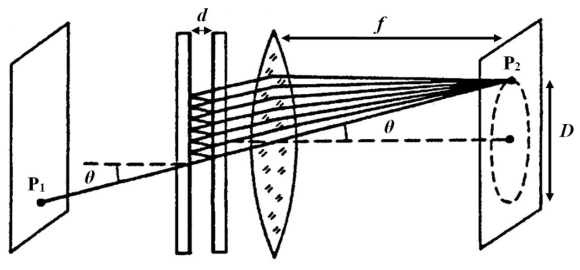
\includegraphics[width=0.75\textwidth]{figure2.png}
    \caption{Illustration of a Fabry-Perot interferometer, including a light path.\cite{manual}}
    \label{fig:FP}
\end{figure}

\begin{figure}[h!]
    \centering
    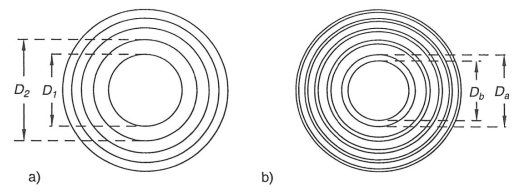
\includegraphics[width=0.85\textwidth]{rings.png}
    \caption{Interference pattern produced by the Fabry-Perot.\cite{manual}}
    \label{fig:FP}
\end{figure}

It can be derived 

\subsection{The Zeeman Effect}
This effect is due to the spin momentum properties of electrons. When exposed to an electric field with magnitude $B$, the normally degenerate energy levels will split according to the relation 

\begin{equation} \label{eq:zeeman}
\Delta E_B = g_J \mu_B B M_J,    
\end{equation}
\noindent
where $g_J = \frac{3}{2} + \frac{S(S+1) - L(L+1)}{2J(J+1)}$ is the Landé factor, $\mu_B$ is the Bohr magneton and $M_J$ is the secondary total angular momentum quantum number.



\subsubsection{Polarization of light}
A non-trivial consequence of the Zeeman effect is that the light emitted from each separate transition will have a well-defined polarization (linear $\pi$ or circular $\sigma^{\pm}$), dependent on the difference in quantum number $M_J$ between energy levels. Also, no $\pi$-polarized light will be emitted in the direction parallel to the magnetic field. \\\\
\noindent

\begin{table}[h!]
\centering
\begin{tabular}{l|l|l}
Transition                      & Wavelength & Color     \\ \hline
5s5p $^1$P$_1$ - 5s5d $^1$D$_2$ & 643.8 nm   & Red       \\
5s5p $^3$P$_2$ - 5s6s $^3$S$_1$ & 508.6 nm   & Green     \\
5s5p $^3$P$_1$ - 5s6s $^3$S$_1$ & 480.0 nm   & Turquoise \\
5s5p $^3$P$_0$ - 5s6s $^3$S$_1$ & 467.8 nm   & Blue     
\end{tabular}
\caption{Table of considered transitions and the respective wavelength of emitted light.\cite{manual}}
\label{tbl:transitions}
\end{table}

If one considers the particular case of Cd emission from the transitions listed in Table \ref{tbl:transitions}, the the energy difference $E - E_0$ in units of $\mu_B B$ can be calculated for each individual transition. Here $E$ and $E_0$ are the energies of the transition under and the influence of a magnetic field, respectively. The results of the calculation are summarized in Table \ref{tbl:polarizations}.

\begin{table}[h!]
\centering
\begin{tabular}{l|l|l|l}
Transition                      & $\pi$                            & $\sigma^+$             & $\sigma^-$          \\ \hline
5s5p $^1$P$_1$ - 5s5d $^1$D$_2$ & 0, 0, 0                            & -1, -1, -1               & 1, 1, 1               \\
5s5p $^3$P$_2$ - 5s6s $^3$S$_1$ & $-\frac{1}{2}$, 0, $\frac{1}{2}$ & -2, $-\frac{3}{2}$, -1 & 1, $\frac{3}{2}$, 2 \\
5s5p $^3$P$_1$ - 5s6s $^3$S$_1$ & -$\frac{1}{2}$, $\frac{1}{2}$    & -2, -$\frac{3}{2}$     & $\frac{3}{2}$, 2    \\
5s5p $^3$P$_0$ - 5s6s $^3$S$_1$ & 0                                & -2                     & 2                  
\end{tabular}
\caption{The considered transitions of Cd along with the polarizations of spectral lines when exposed to a magnetic field. The values in each cell gives the energy difference of each transition in units of $\mu_B B$ (hence a dimensionless quantity).}
\label{tbl:polarizations}
\end{table}


\subsection{Error estimation and instrument}


\section{Method}
The lab setup of the lab consisted of one cadmium light source placed inside an electromagnet, all of which was placed on a rotating table. The output of the lamp  Next to the table was mounted, in successive order from the light source, a 50mm lens, a Fabry-Perot interferometer, a 300mm lens, a 50mm lens and a CCD-camera. Also used during the lab was color filters of wavelengths 480nm, 595nm, 470nm, 508nm, a linear polarizer and a quarter-wave plate. \\

\begin{figure}[h]
    \centering
    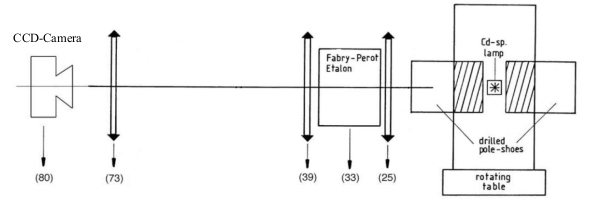
\includegraphics[width=0.9\textwidth]{figure1.png}
    \caption{Illustration of the setup. The number in parenthesis under each instrument indicates its approximate distance from the light source in centimeters.\cite{manual}}
    \label{fig:setup}
\end{figure}

\noindent
After calibration, the table was rotated so that only the  the polarization of the light from the Cd source was investigated. The polarizer and quarter-wave plate were mounted between the second and third lenses in the succession. By rotating the wave plate and filtering a certain polarization with the polarizer, the circular polarization of the emitted light could be deduced. Each group of transitions could be considered individually by placing a color filter after the second lens.\\
\noindent
Next, the wave plate and polarizer were removed and pictures of the wave pattern output of the Fabry-Perot were captured by the CCD-camera. 
This was done for each of the four major wavelengths with the use of color filters, as well as magnetic field magnitudes ranging from $0$ T to $3$ T with increments of $0.5$ T.
\section{Results}
\subsection{Qualitative Results}
When looking at the different transitions from the longitudinal direction (parallel to the magnetic field) with the magnetic field on, it was noted that some of the lines observed when looking at the lines from the transverse direction were missing. The missing lines correspond to the $\pi$ transitions, whose light does not propagate in the direction parallel to the magnetic field due to their linear polarization.\\
\begin{figure}[H]
    \centering
    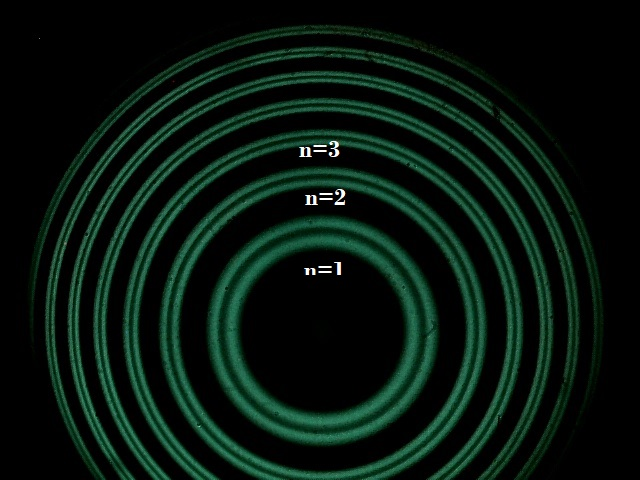
\includegraphics[width=0.6 \textwidth]{Lines.jpg}
    \caption{Zeeman splitting of the turquoise line (480 nm)  in the longitudinal direction under a magnetic field of $0.3$ T. There are two rings for every interference order $n$, one belongs to a $\sigma^+$ transition and the other to a $\sigma^-$ transition.}
\end{figure}
\noindent
When looking at the transition lines from the longitudinal direction with the wave plate and the linear poralizer in place, it was possible to separate the $\sigma^+$ transitions from the $\sigma^-$ transitions. When the wave plate was rotated by $\frac{\pi}{2}$ the linear polarizer could be used to filter out one of the $\sigma$ transitions. It was observed that when the linear polarizer was at $\frac{\pi}{4}$ both $\sigma$ transitions had similar intensities. However, as the linear polarizer was rotated towards $\frac{\pi}{2}$ it was observed that one of the lines faded out until it was almost unnoticeable. The same effect was observed when turning the polarizer towards $0$ but with the role of the lines inverted. This is caused by the effect of the wave plate on circularly polarized light; as circularly polarized light passes through the wave plate it becomes linearly polarized light, this linearly polarized light can then be filtered using a linear polarizer. Due to the difference in direction of polarization of the $\sigma^+$ and $\sigma^-$ transitions, one of them becomes vertically polarized and the other one horizontally polarized after passing through the wave plate. 


\subsection{Quantitative Results}
In order to have an idea of the accuracy of the experimental measurements, the theoretical slope of the Zeeman splitting against the magnetic field was calculated using equation ():
$$
\Delta \sigma=  \frac{E_{mag}}{hc}=2\frac{g_J \mu_B B M_J}{hc}
$$
\begin{equation}
   \Delta \sigma_{\text{blue}}^{\text{theo}}= \frac{4\mu_B}{hc} B = 186.74  \ \ m^{-1} \  B= 1.87  \ \ cm^{-1} \  B
\end{equation}

\begin{equation}
   \Delta \sigma_{\text{red}}^{\text{theo}}= \frac{2\mu_B}{hc} B = 93.37 \ \ m^{-1} \  B= 0.93  \ \ cm^{-1} \  B
\end{equation}
The experimental Zeeman splitting was calculated using the collected data and equation(). The plots of both the theoretical and experimental Zeeman splittings for the red (643.8 nm) and blue (467.8 nm) lines are shown in Figures () and ().\\

\begin{equation}
    \Delta \sigma_{\text{blue}}^{\text{exp}}= 2.49 \pm 0.06 \ cm^{-1}
\end{equation}
\begin{equation}
    \Delta \sigma_{\text{red}}^{\text{exp}}= 1.23 \pm 0.05 \  cm^{-1}
\end{equation}
It is possible to eliminate the need to accurately know the thickness $d$ between the plates in the Fermy-Perot by considering the ratio $R$ between the slopes of two lines rather than their individual slopes. This ratio can then be compared to the ratio of the theoretical slopes calculated in equations () and ().
\begin{equation}
    R_{theo}= \frac{1.87 \ \ cm^{-1}}{0.93\ \ cm_{-1}}= 2.00
\end{equation}
The experimental ratio was obtained by taking the average value of the ratio between the Blue and Red Zeeman splittings, given by equation ():

\begin{equation}
    R_{exp}= \overline{\left( \frac{\Delta \sigma_{Blue}}{\Delta \sigma_{Red}} \right)} = 2.00
\end{equation}





\begin{figure}[H]
    \centering
    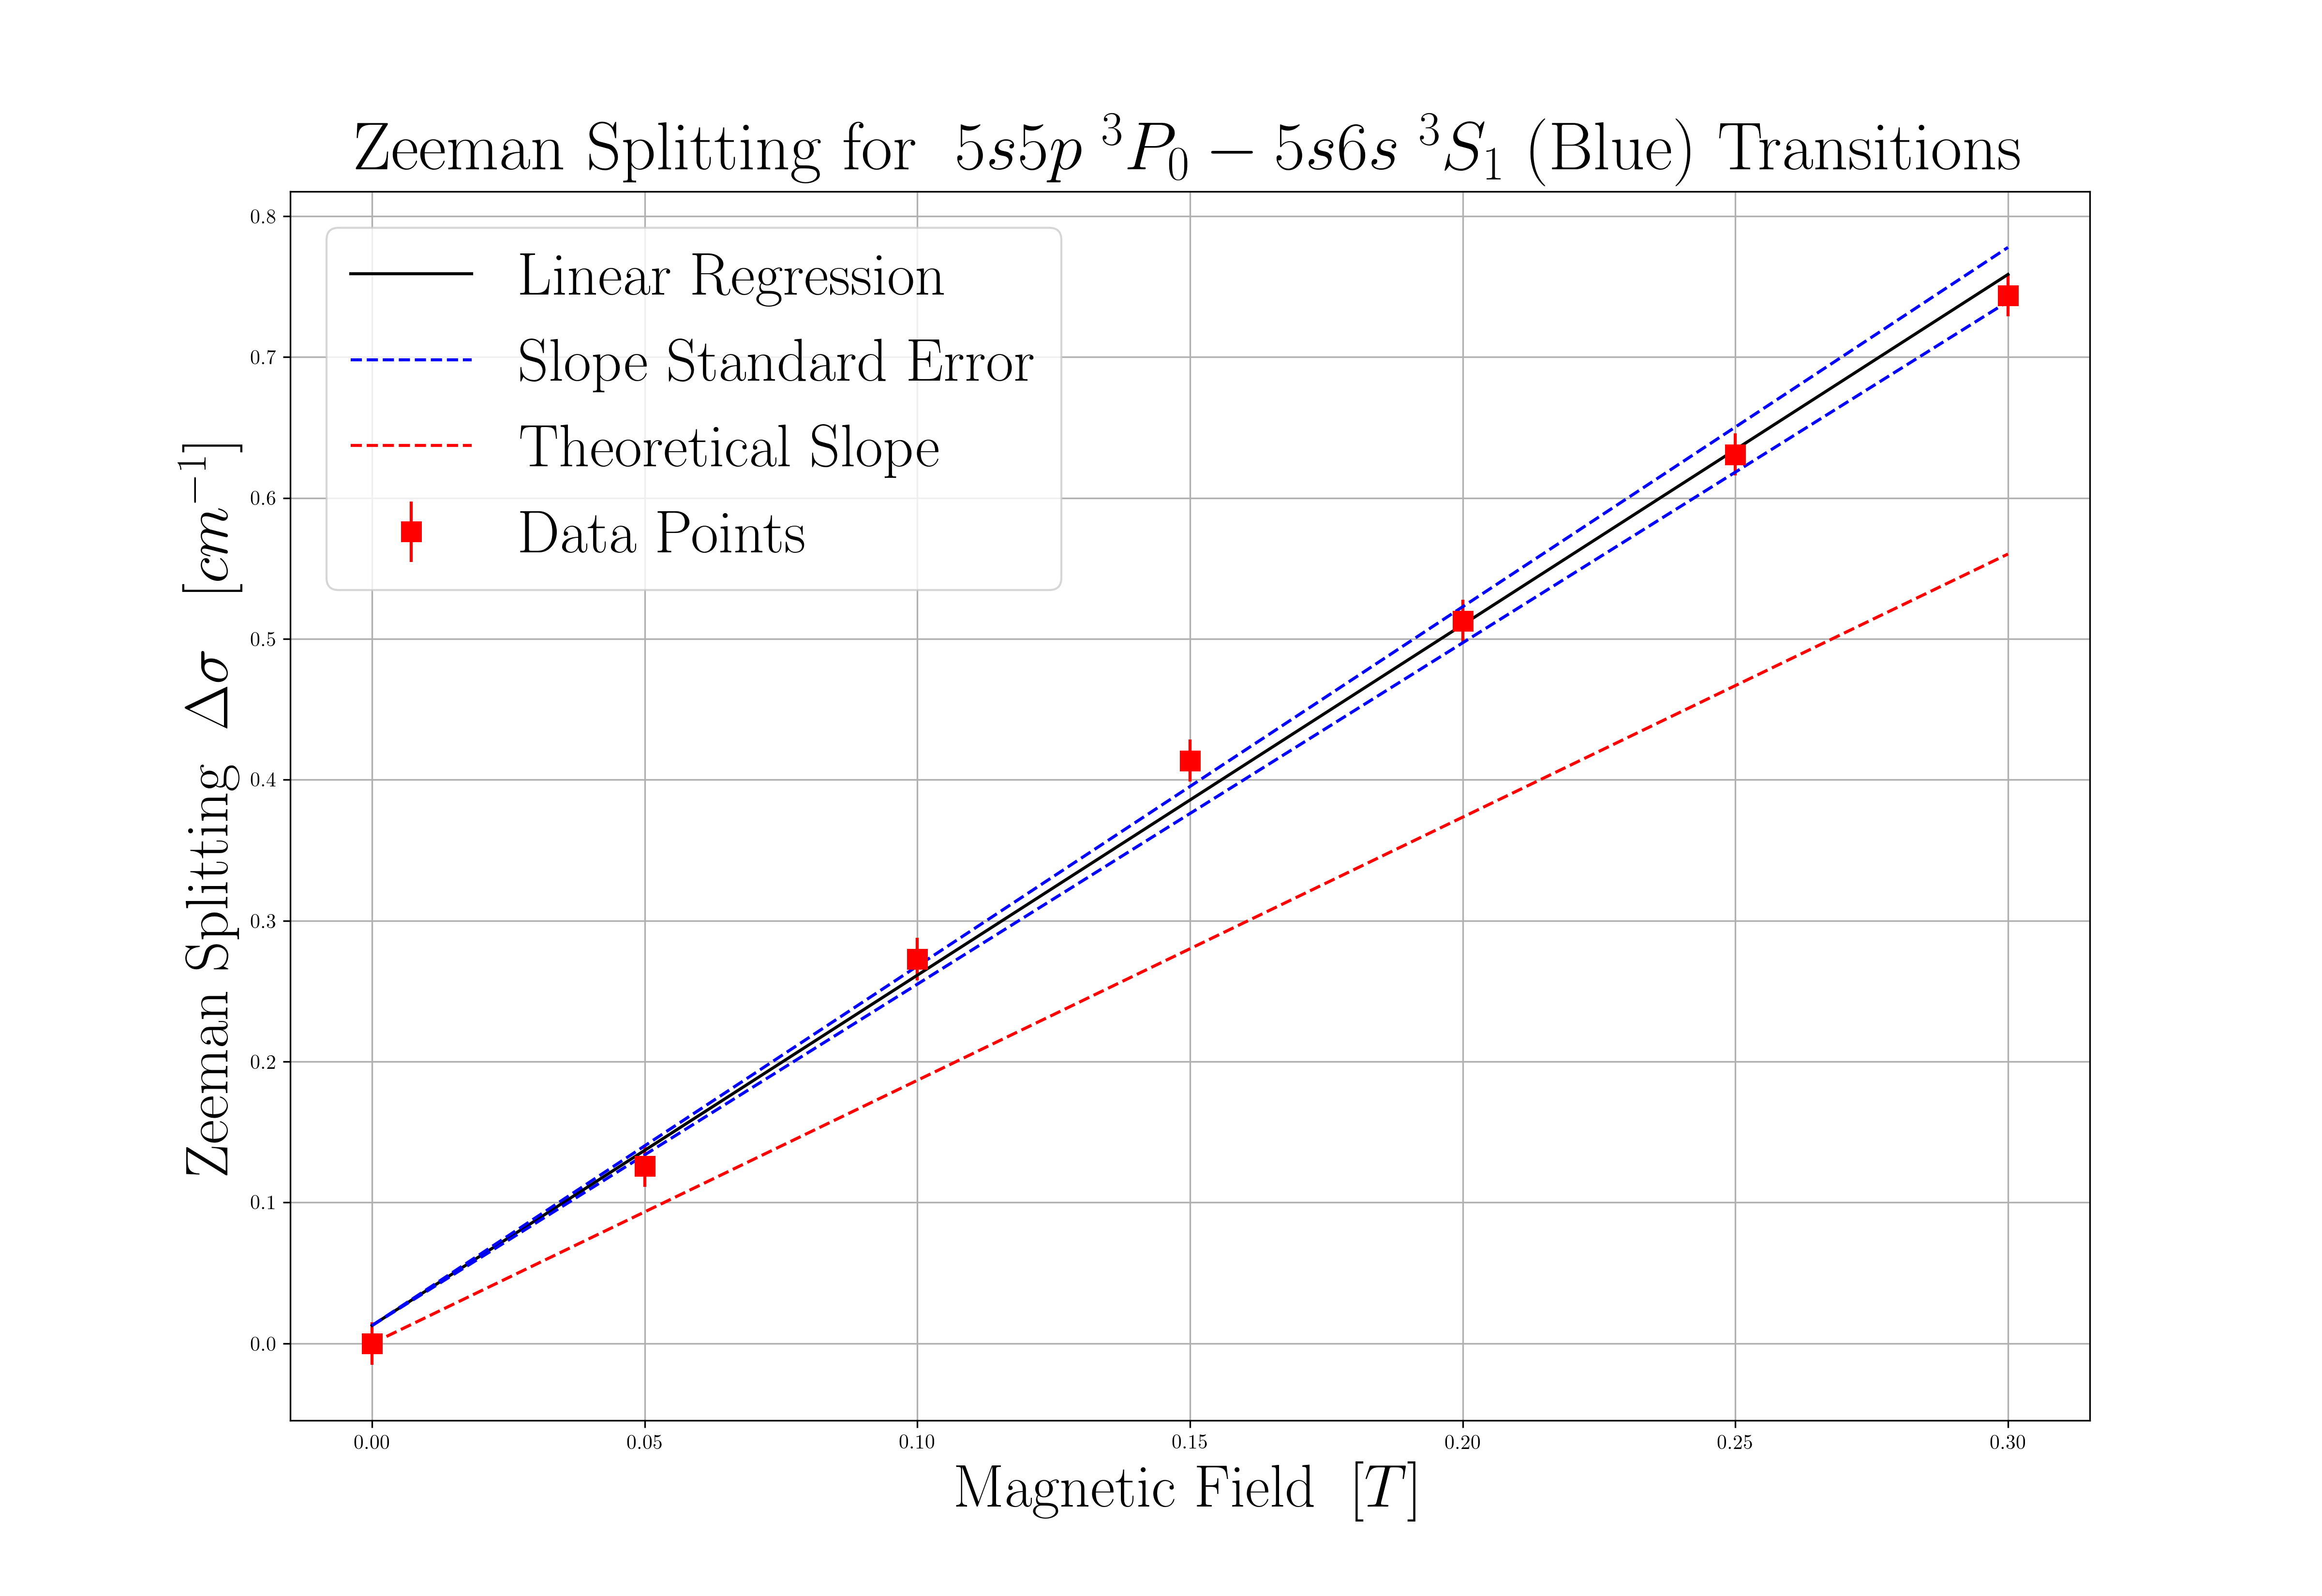
\includegraphics[width=1 \textwidth]{BlueSlope.png}
    \caption{ Zeeman splitting against magnetic field for blue line ($470$ nm) in Cadmium. A linear regression was obtained from the data points and the Standard error on the slope due to the uncertainty on the data was included.}
\end{figure}

\begin{figure}[H]
    \centering
    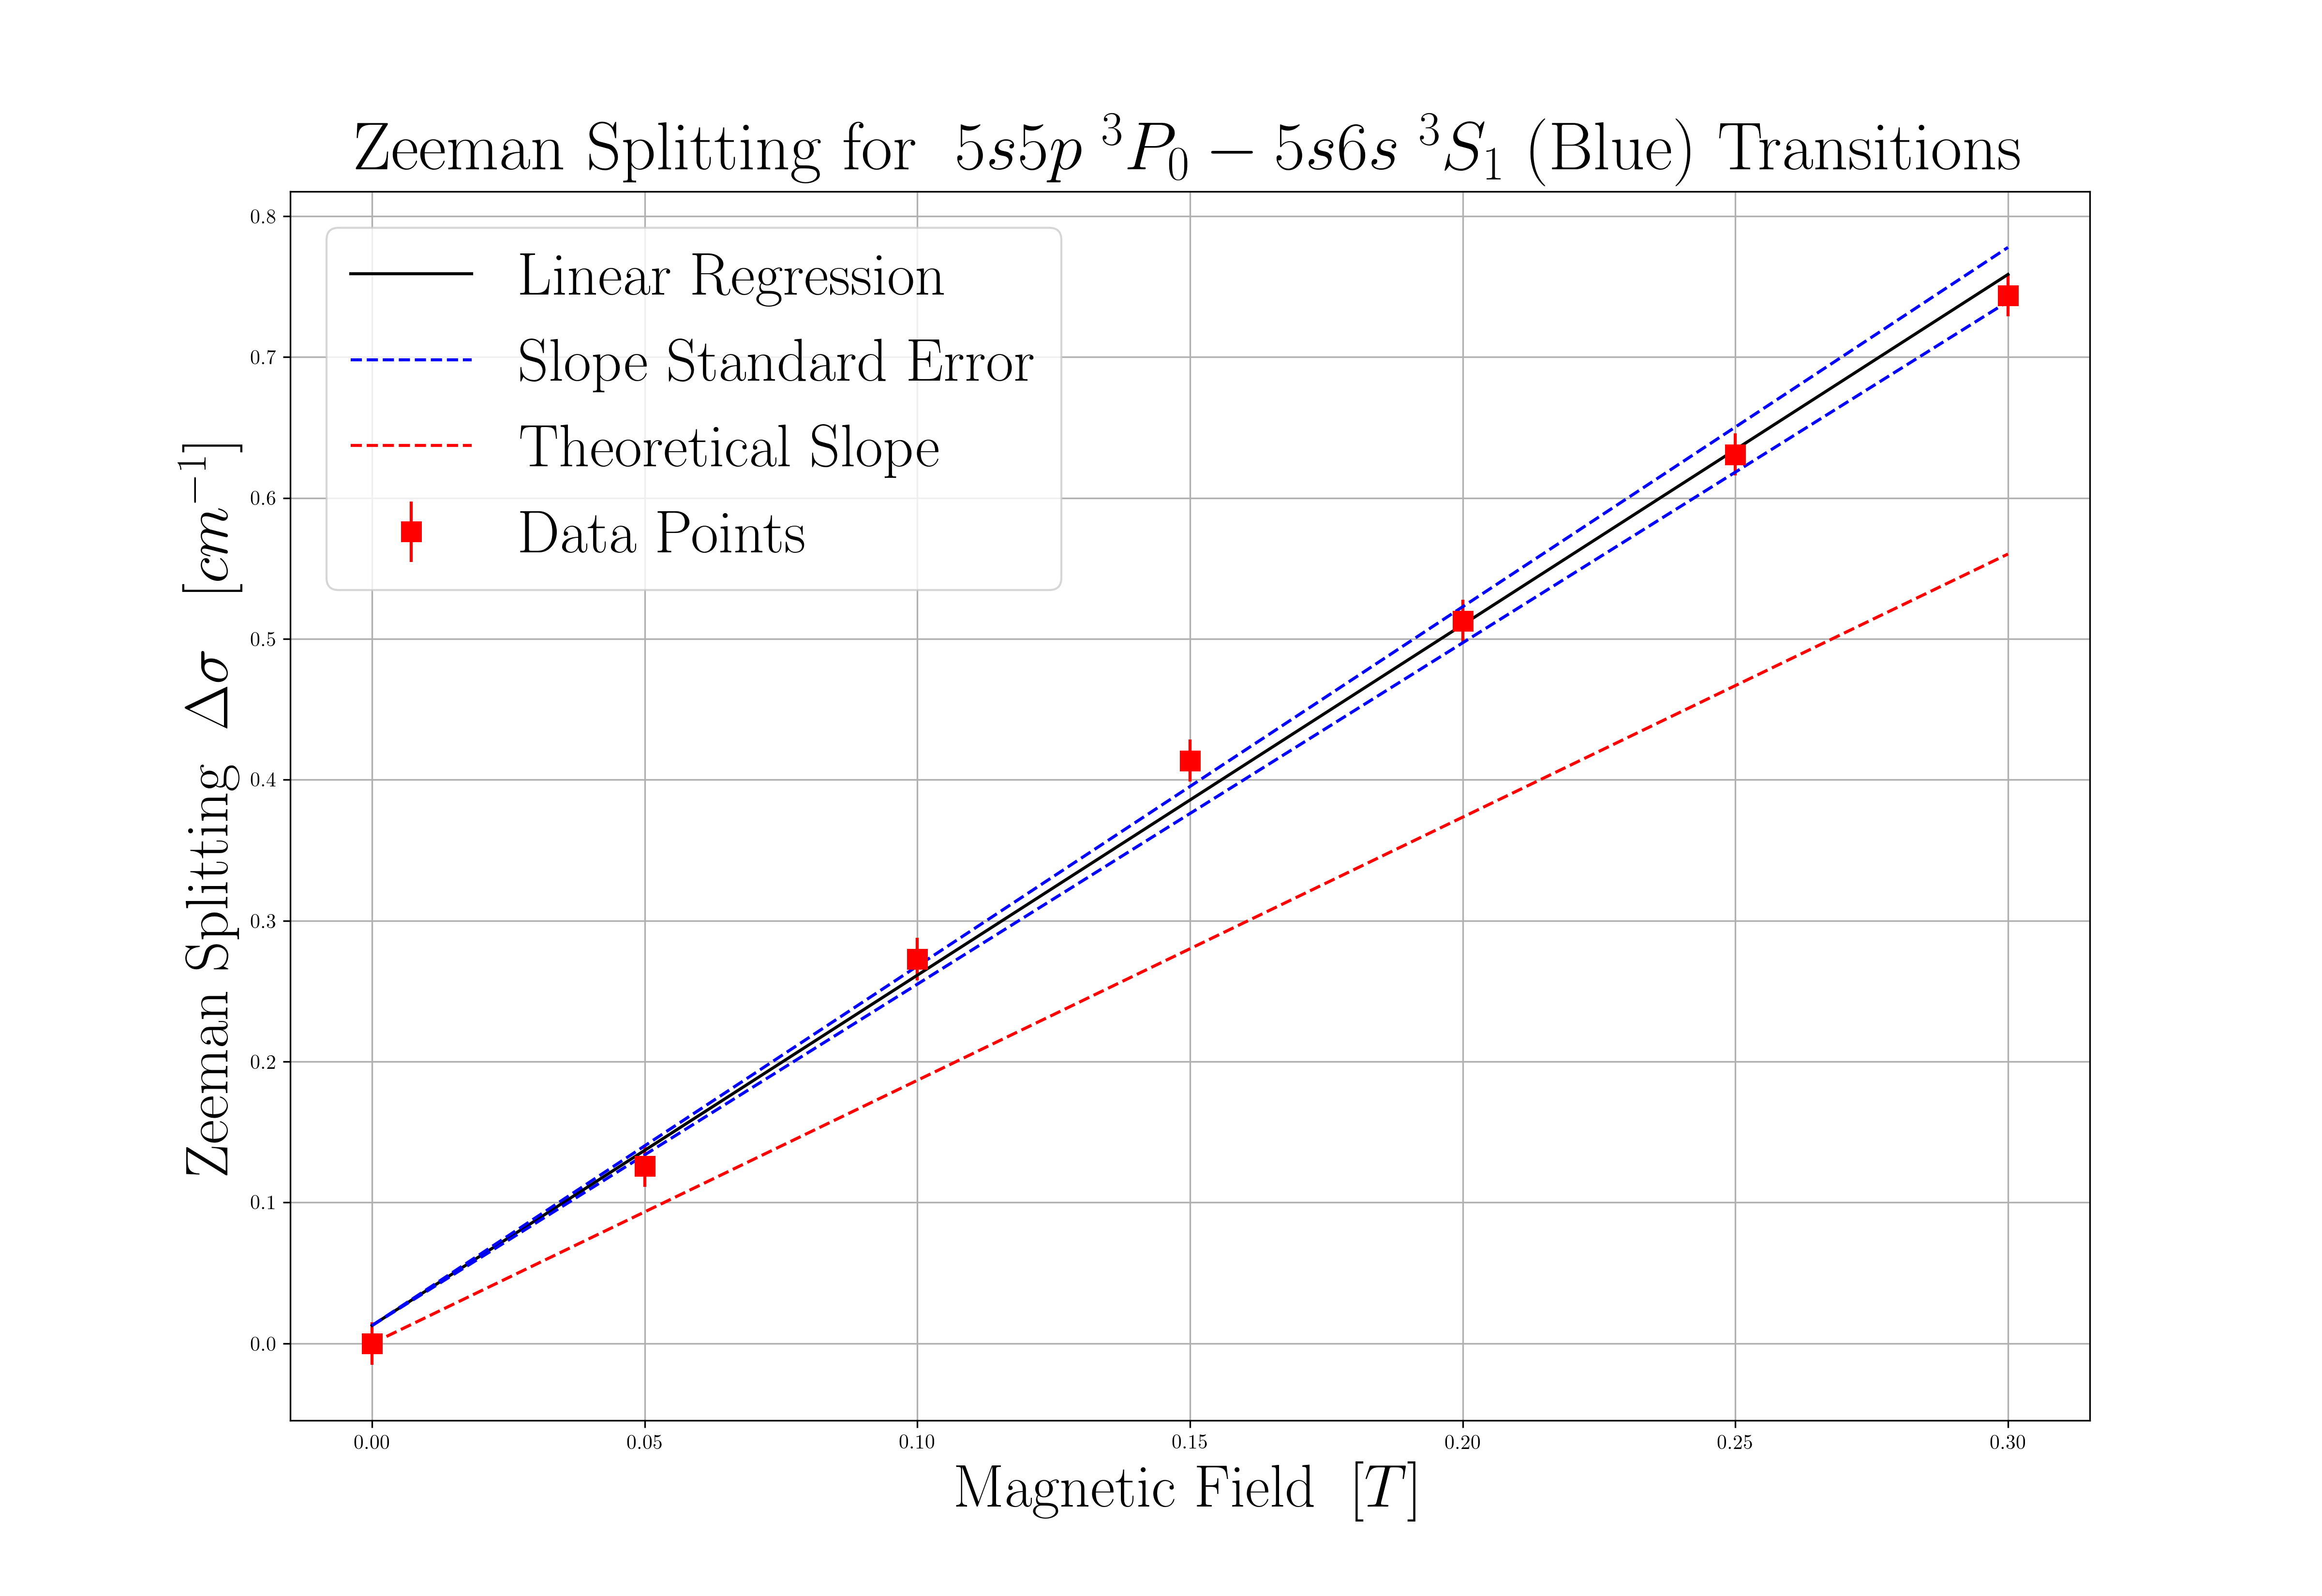
\includegraphics[width=1\textwidth]{BlueSlope.png}
    \caption{Zeeman splitting against magnetic field. This plot corresponds to the red ($643.8$ nm)  line in Cadmium.}
\end{figure}

\section{Discussion}
Very important properties of the transitions in cadmium were observed during the laboratory session. We observed that by looking at the lamp from different directions it was possible  to determine the existence of perfectly linearly polarized emission light, such as in the case of $\pi$ transitions. However, for some lines such as the green line, this effect was not completely evident,

\begin{thebibliography}{99}
\bibitem{manual}
Department of Physics, 2018-02-06, FYSC11 Lab Manual: \textit{The Zeeman Lab}, Lund University

\end{thebibliography}

\end{document}
